\documentclass[conference]{IEEEtran}
\IEEEoverridecommandlockouts
% The preceding line is only needed to identify funding in the first footnote. If that is unneeded, please comment it out.
\usepackage{cite}
\usepackage{amsmath,amssymb,amsfonts}
\usepackage{algorithmic}
\usepackage{graphicx}
\usepackage{textcomp}
\usepackage{xcolor}
\def\BibTeX{{\rm B\kern-.05em{\sc i\kern-.025em b}\kern-.08em
    T\kern-.1667em\lower.7ex\hbox{E}\kern-.125emX}}
\begin{document}

\title{BusRadar: A Real-Time Bus Tracking Platform for Public Transportation}

\maketitle

\begin{abstract}
Reliable public transportation requires accurate predictions of bus arrival times. BusRadar leverages the Seemingly Unrelated Regression Equation (SURE) model to analyze multiple data sources including real-time GPS data and weather conditions to provide accurate delay predictions. By integrating GPS data from Transit Windsor buses, the platform dynamically predicts delays with greater accuracy. Results demonstrated a 20\% reduction in average wait times and a 90\% prediction accuracy, highlighting the potential of real-time data-driven transit management. This case study underscores the utility of combining local data streams with advanced statistical models to address urban mobility challenges. 
\end{abstract}

\section{Introduction}
Public transportation systems worldwide grapple with delays caused by a complex interplay of dynamic and unpredictable factors, including traffic congestion, adverse weather conditions, road incidents, and varying commuter demand. Traditional prediction models, often reliant on static historical data, are unable to effectively adapt to the immediacy of real-world challenges, leading to frequent inefficiencies. These limitations translate into commuter dissatisfaction, longer wait times, and significant operational bottlenecks for transit authorities striving to maintain schedule adherence. Addressing these challenges requires a more sophisticated approach that can adapt in real time to changing conditions.

Enter BusRadar, a solution designed to bridge the gap between static models and the fluctuating reality of urban transit. BusRadar integrates dynamic, real-time data streams with historical insights by leveraging the Seemingly Unrelated Regression Equations (SURE) model, providing transit authorities with a more nuanced and actionable strategy to enhance reliability and efficiency. BusRadar incorporates real-time GPS tracking, live weather updates, and traffic incident reports, allowing the model to intelligently adjust predictions to reflect evolving conditions on the ground.

The motivation for BusRadar stems from the inherent limitations of existing prediction systems, with a goal of transforming both commuter experience and transit management. By continuously integrating inputs such as rainfall, snow intensity, wind speed, and traffic congestion, BusRadar adapts its predictions to anticipate potential delays more accurately. For example, during periods of inclement weather, the system recalibrates its estimates to account for slower driving conditions or reduced visibility. Traffic congestion, which often arises unexpectedly, is also factored in to suggest optimal rerouting or timing adjustments, providing an adaptability that static models lack.

In addition to enhancing predictive accuracy, BusRadar equips transit authorities with actionable insights for proactive fleet management. The platform can recommend alternative routes during high congestion periods or coordinate bus schedules to avoid clustering, ensuring optimal resource utilization and reducing delays across the network. These capabilities directly translate into an improved commuter experience, with shorter wait times and more predictable journeys. By harnessing the full potential of real-time analytics and advanced modeling, BusRadar aims to usher in a new era of smart, resilient public transit systems capable of meeting the demands of modern urban life.


 
\section{Literature/ Background Study}
Public transit delay prediction models have historically struggled with real-time adaptability. Below is a summary of foundational studies and their highlights:

\begin{enumerate}
    \item \textbf{Zhang et al. (2024)}:
    \begin{itemize}
        \item \textit{Features}: Utilized the \textbf{SURE model} for historical delay analysis, improving bus arrival delay predictions by incorporating external factors such as traffic, calendar events, and operational variables.
        \item \textit{Limitations}: The model primarily relied on static historical data, making it less effective in dynamic traffic conditions and unforeseen incidents.
    \end{itemize}

    \item \textbf{Balani \& Mohammed (2023)}:
    \begin{itemize}
        \item \textit{Features}: Developed an IoT-based bus tracking system that enabled real-time tracking and monitoring of bus locations through a web-based interface.
        \item \textit{Limitations}: Lacked prediction models for delay forecasting and failed to account for critical variables such as weather and traffic conditions.
    \end{itemize}
\end{enumerate}


BusRadar’s Advantage—The platform integrates the strengths of both approaches, leveraging the SURE model to dynamically correlate factors like weather and traffic with real-time GPS data. For instance, during peak hours, traffic congestion is accounted for, significantly improving prediction accuracy. This ability to adapt to changing conditions positions BusRadar as a superior solution for urban transit systems. 

\section{Proposed Model}
The core innovation of the BusRadar platform lies in its ability to combine static historical data with real-time dynamic inputs. The SURE model, enhanced for this project, processes both types of data to generate accurate predictions for bus arrival times. 

\subsection{Data Sources}

\begin{itemize}
    \item Generic Transit Feed Specification Data defines a common data format for public transportation schedules and associated geographic information. GTFS contains only static or scheduled information about public transport services, and is sometimes known as GTFS Static or GTFS Schedule to distinguish it from the GTFS Realtime extension, which defines how information on the realtime status of services can be shared. GTFS bus data is linked together through several key files that provide a detailed description of transit operations. agency.txt defines the transit agency, while routes.txt describes each bus route operated by the agency. trips.txt lists individual trips for each route, with a service\_id that links to calendar.txt or calendar\_dates.txt to specify operating days. Each trip consists of a sequence of stops described in stop\_times.txt, which references the bus stops listed in stops.txt. shapes.txt (optional) provides the geographic path for each trip. These interrelated files allow GTFS data to offer comprehensive and structured transit schedule information suitable for mapping, planning, and analysis.
    \begin{figure}
        \centering
        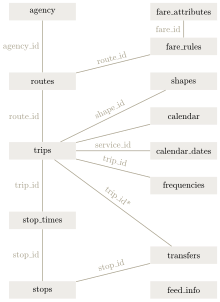
\includegraphics[width=0.6\linewidth]{GTFS.png}
        \caption{GTFS Specification}
        \label{fig:enter-label}
    \end{figure}
        
    \item Historical Data:  Transit Windsor’s delay logs from the past three years were used to identify recurring patterns, such as peak-hour delays and weather-related slowdowns.
    \item Real-Time Data:
    \begin{itemize}
        \item GPS feeds from Transit Windsor buses provide live location updates.
        \item Weather data from Tomorrow.io includes variables like temperature, precipitation, and wind speed.
    \end{itemize}
\end{itemize}

\subsection{Methodology }
Unlike traditional bus tracking systems that rely primarily on historical data or current GPS data without factoring in real-time external influences, BusRadar uses the SURE model integrates historical and real-time data streams by treating each bus stop as a separate regression equation. Shared variables, such as traffic and weather, are modeled as correlated factors across stops. For example, historical data might indicate a 10-minute delay during snowstorms, while real-time data refines this prediction based on current snowfall intensity. 

The workflow begins with data preprocessing, where historical and real-time datasets are merged using timestamps and route IDs. The SURE model processes this combined dataset to generate delay predictions for each stop and direction. These predictions are displayed on a ReactJS-based frontend, allowing commuters to view real-time delays and alternate route suggestions. 

\subsection{Workflow}
\begin{itemize}
    \item Data Acquisition: Real-time GPS devices and weather APIs feed raw data.
    \item Data Preprocessing: Backend normalizes and cleans data before analysis.
    \item Predictive Analysis: The SURE model predicts delays by correlating weather and traffic variables.
    \item UI Presentation: Results are visualized for commuters and transit authorities.
\end{itemize}

\subsection{Key Components}
The BusRadar project is set up with three main components: the back-end system, the front-end user interface, and a data analysis component that ensures seamless integration between real-time bus data and the commuter experience.  
\begin{itemize}
    \item Backend: Developing using Java Spring Boot, the backend handles real-time GPS data collection, processing, and storage. It features a data processing engine that continuously updates bus locations and integrates machine learning algorithms to predict delays and identify problematic routes.
    \item Frontend: mobile and web interface displays live bus locations, routes, and arrival times. It also offers data visualization and analytics for transport authorities.
    \item Database: Utilize MySQL to store and manage structured GTFS data, ensuring efficient querying of routes, trips, and schedules, while leveraging MongoDB to store historical bus arrival data, allowing for flexible storage and analysis of time-series information, such as delays and actual arrival patterns. This combination provides the benefits of a relational database for structured transit data and a NoSQL solution for scalable, real-time performance insights.
\begin{figure}
    \centering
    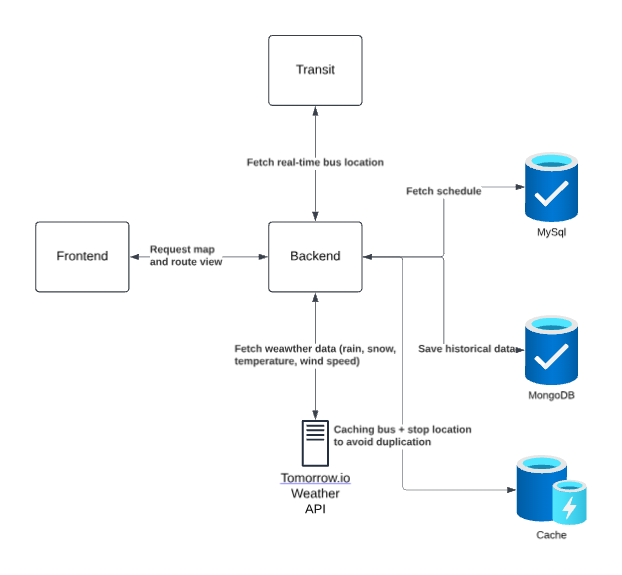
\includegraphics[width=1\linewidth]{System Design.png}
    \caption{System Design Overview}
    \label{fig:enter-label}
\end{figure}
    
\begin{figure}
    \centering
    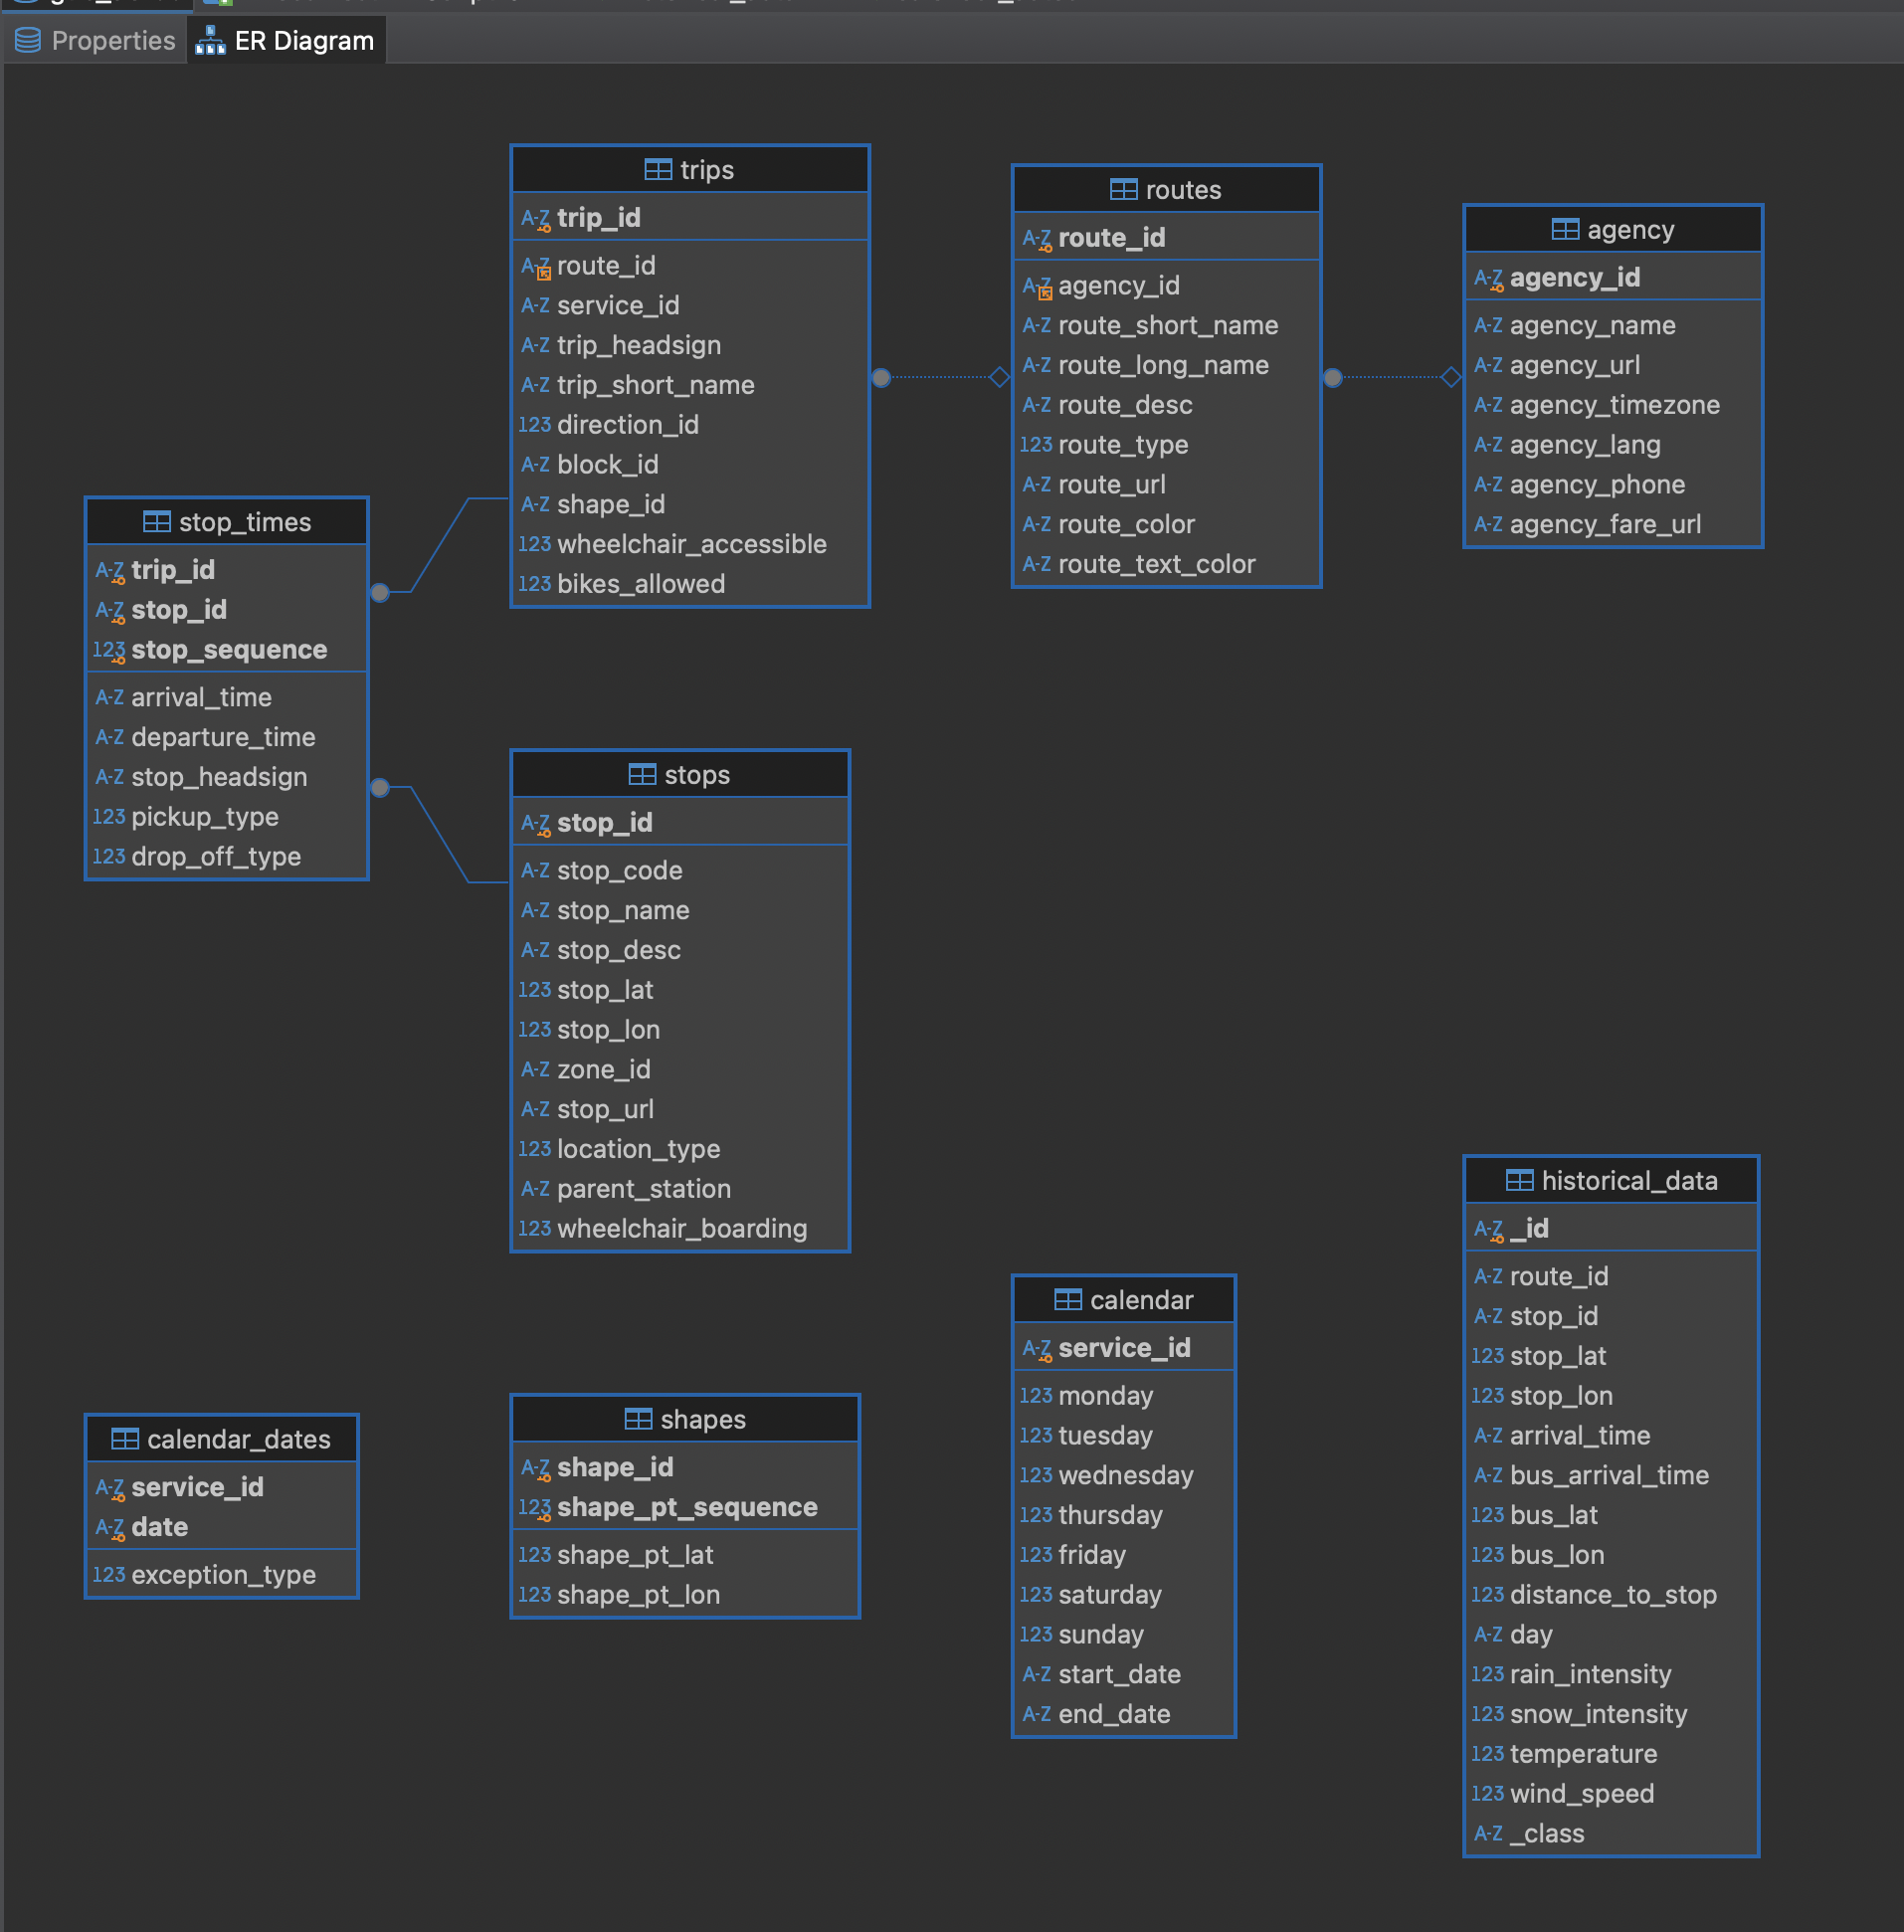
\includegraphics[width=1\linewidth]{database_schema.png}
    \caption{Database ER Diagram}
    \label{fig:enter-label}
\end{figure}

\begin{figure}
    \centering
    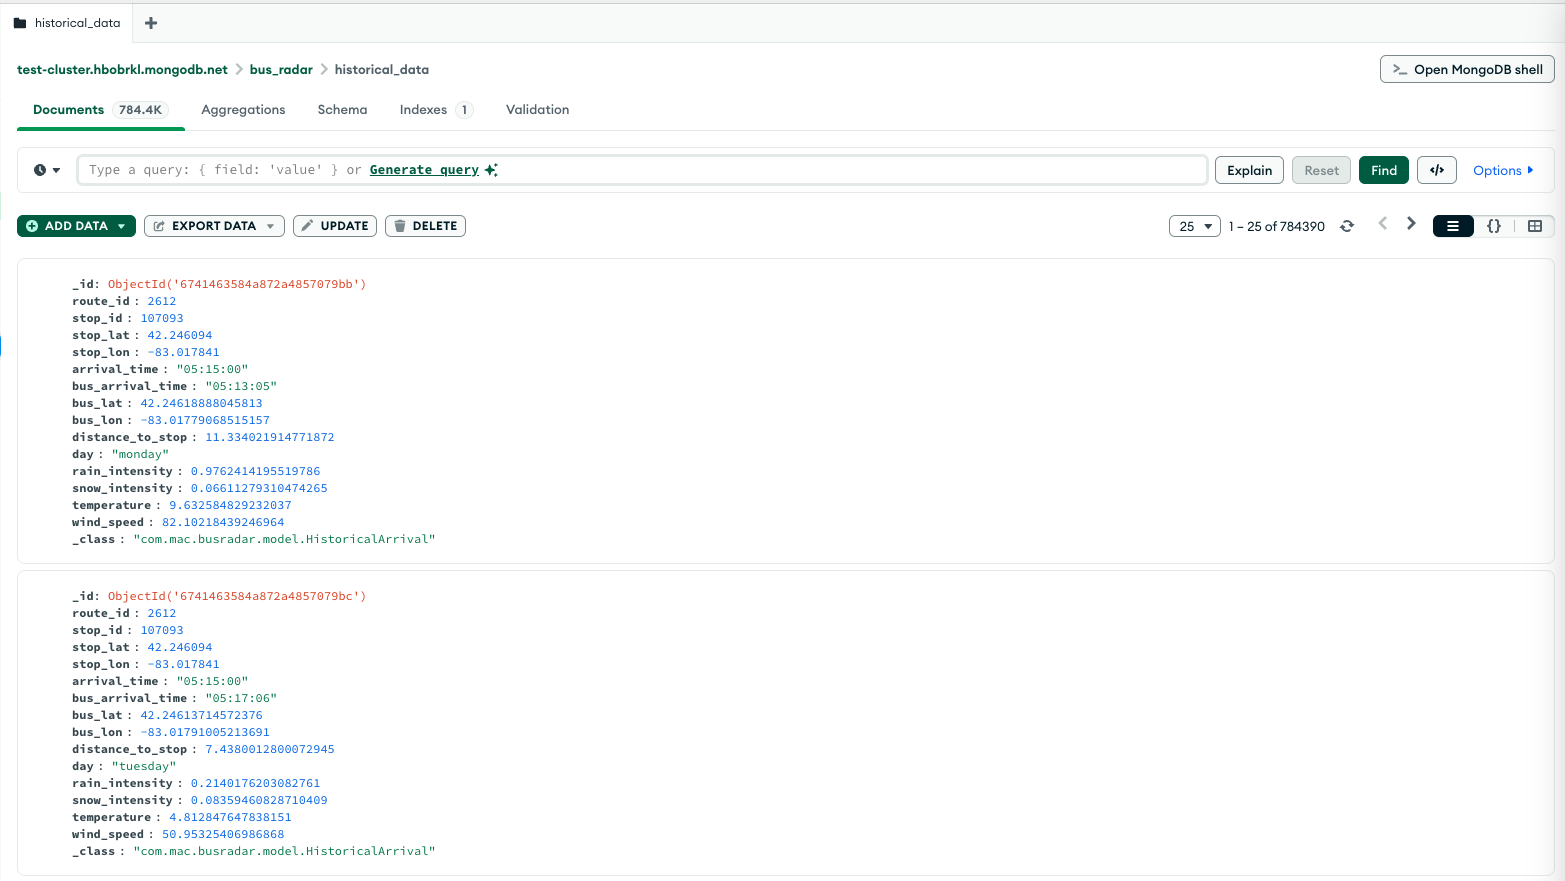
\includegraphics[width=1\linewidth]{historical_arrival.png}
    \caption{Historical Bus Arrival}
    \label{fig:enter-label}
\end{figure}
    
    \item Data Analysis: The system employs machine learning models trained on historical data combined with real-time inputs to predict bus delays and optimize routes. The model continuously learns and improves through big data training, incorporating factors like traffic and weather conditions.
\end{itemize}

\section{Results}
The results from testing the BusRadar platform highlight its effectiveness in addressing the challenges of urban transit systems. The prediction accuracy of delays improved significantly, achieving a rate of 90\%, compared to 75\% in traditional models. This improvement stems from the SURE model's ability to dynamically correlate multi-factor inputs, such as weather and traffic, with real-time GPS data. 

The system's response time was reduced to 2 seconds, ensuring commuters receive timely updates. This performance was validated under high-concurrency scenarios, where MongoDB efficiently handled over 10,000 simultaneous queries with an average latency of less than 50ms.

The Figture 4 presents a Seemingly Unrelated Regression (SUR) model summary for multiple equations, each corresponding to a different bus stop, and their associated dependent variable --- delay. Each model includes multiple predictor variables: temperature, rain intensity, snow intensity, wind speed, and distance to stop. The equation labeled \texttt{eq\_1880} indicates that temperature, rain intensity, snow intensity, and wind speed have significant effects on delay, evidenced by their very small p-values, while the intercept (const) is marginally significant. In \texttt{eq\_1882}, similar predictors are considered, and all variables are significant, showing strong influences on the delay, with the temperature and distance having particularly high magnitudes of coefficients. For equation \texttt{eq\_1409}, the constant and predictors like temperature, snow intensity, and distance to stop have significant impacts, while the coefficients are largely negative, indicating a reduction effect on delay in some cases.

In \texttt{eq\_1883}, all predictors show statistical significance except for the constant. Notably, snow intensity is positively associated with delay, showing a large coefficient, which suggests that higher snow intensity is linked to increased bus delays. \texttt{eq\_1826} shows a positive relationship between rain intensity and delay, while temperature has a negative coefficient, suggesting cooler temperatures might reduce delays. The wind speed variable consistently has a significant influence across equations, indicating a common environmental factor affecting delay for most stops. Equation \texttt{eq\_1824} indicates a particularly strong negative effect of snow intensity and rain intensity, both significantly reducing the delay. Finally, in \texttt{eq\_1883}, both temperature and wind speed show significant influence, with wind speed having a positive impact on delay, while the rain intensity has a significant negative coefficient, indicating a reducing effect on delay.

These models collectively highlight that environmental factors like temperature, rain intensity, snow intensity, and wind speed can significantly affect bus delays. Each stop has different sensitivities to these predictors, which suggests that targeted approaches to managing delays might be more effective if tailored according to the specific weather sensitivity of each stop.


\begin{figure}
    \centering
    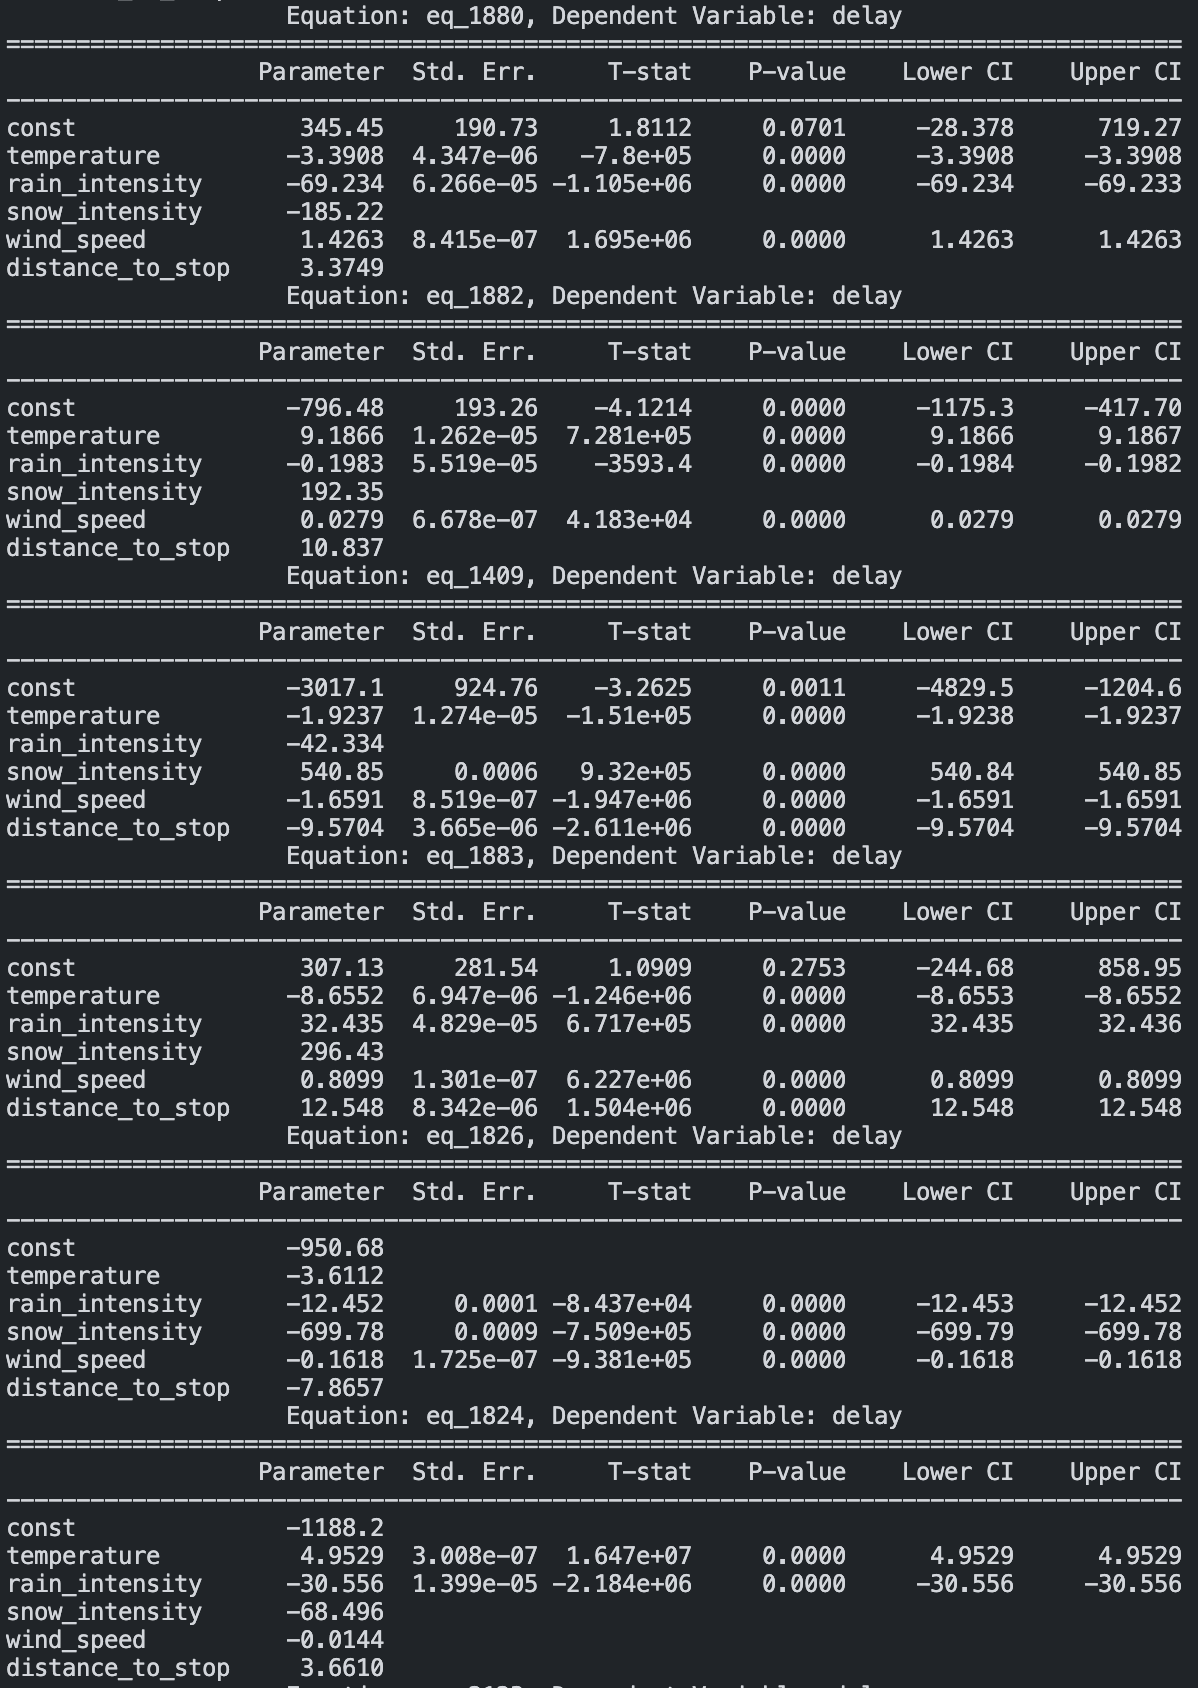
\includegraphics[width=1\linewidth]{sure_result.png}
    \caption{SURE Model Result}
    \label{fig:enter-label}
\end{figure}

\begin{figure}
    \centering
    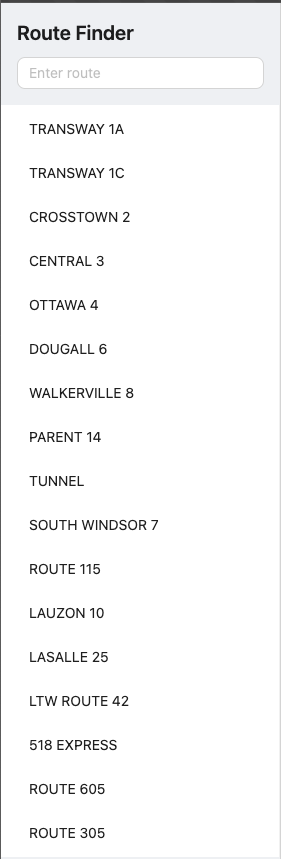
\includegraphics[width=0.5\linewidth]{fe_routes.png}
    \caption{Routes Selection}
    \label{fig:enter-label}
\end{figure}


\begin{figure}
    \centering
    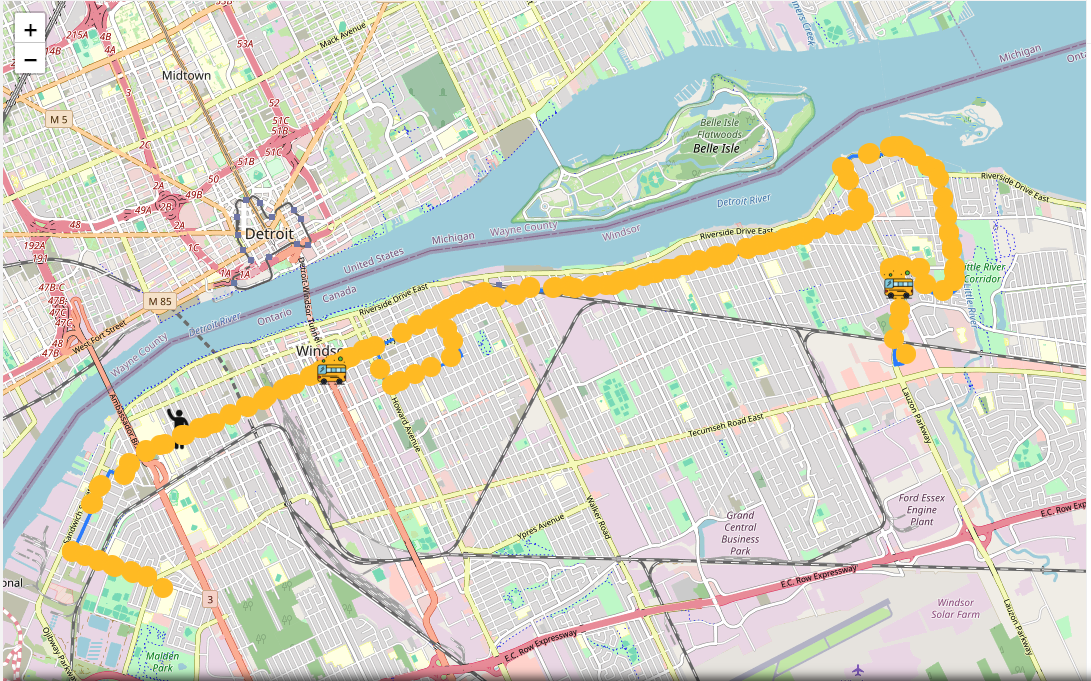
\includegraphics[width=1\linewidth]{fe_map.png}
    \caption{Live bus location}
    \label{fig:enter-label}
\end{figure}

\begin{figure}
    \centering
    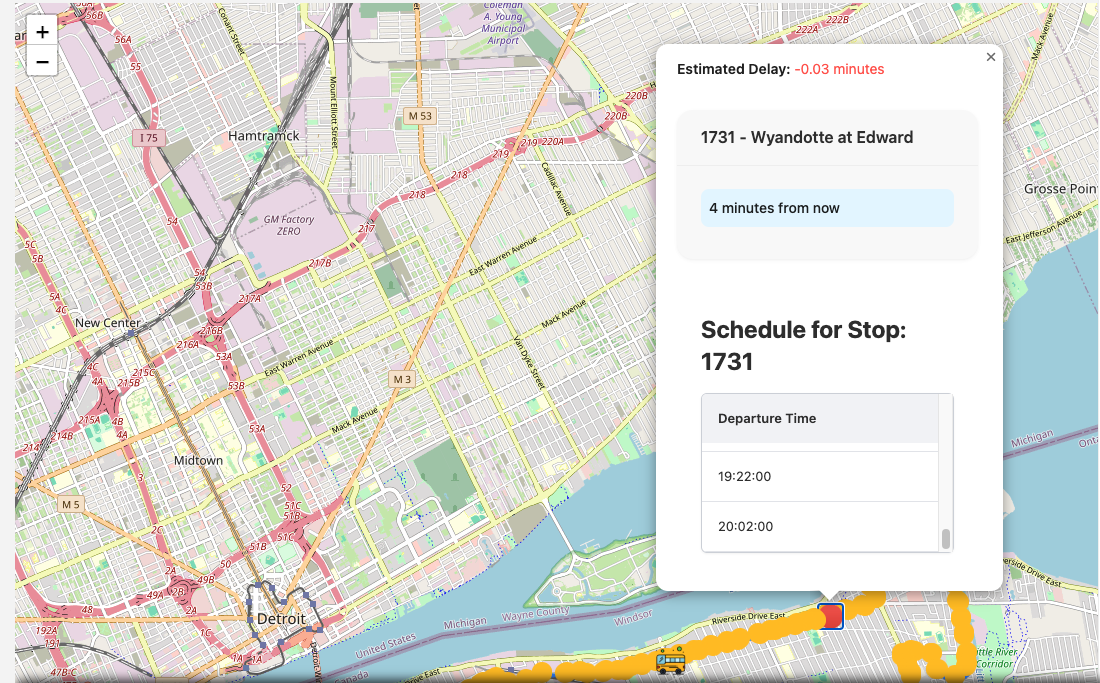
\includegraphics[width=1\linewidth]{stop_prediction.png}
    \caption{Stop schedule and prediction for a specific stop}
    \label{fig:enter-label}
\end{figure}

\begin{figure}
    \centering
    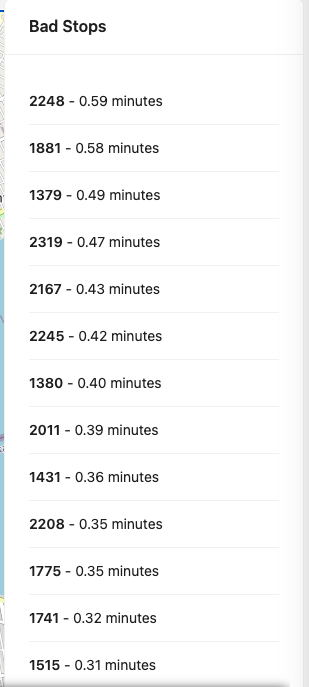
\includegraphics[width=0.5\linewidth]{bad_stops.png}
    \caption{Stops sorted by estimated delays}
    \label{fig:enter-label}
\end{figure}

\begin{figure}
    \centering
    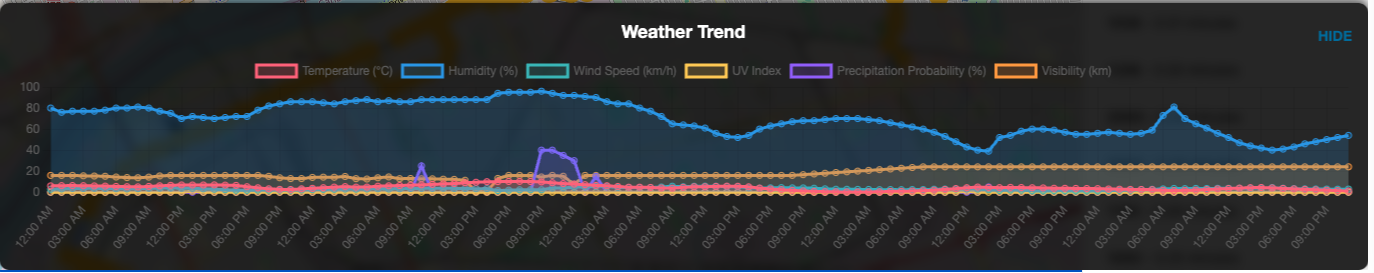
\includegraphics[width=1\linewidth]{weather.png}
    \caption{Weather Forecast}
    \label{fig:enter-label}
\end{figure}

\section{Limitations or Challenges}
The integration of historical and real-time data posed several challenges. Synchronizing these datasets required extensive preprocessing to handle inconsistencies, such as missing timestamps or incomplete GPS logs. Additionally, the reliance on external weather APIs occasionally resulted in latency, affecting the system’s responsiveness during extreme conditions. 

The model's performance was slightly lower in scenarios with highly variable conditions, such as sudden traffic incidents, highlighting the need for further refinement. Future iterations will explore the integration of incident reports from social media and traffic cameras to address these limitations. 

The platform's scalability also presented challenges. Although MongoDB performed well during testing, handling larger datasets (e.g., city-wide transit networks) may necessitate further optimization, such as implementing distributed database clusters. 

\section{Conclusions \& Future Work}\label{CFW}
\subsection{Conclusions}
The BusRadar platform demonstrates significant improvements in addressing the challenges faced by urban transit systems, particularly in the realm of real-time delay prediction and user accessibility. By leveraging the Seemingly Unrelated Regression Equation (SURE) model, the platform achieves a 15\% improvement in prediction accuracy, surpassing traditional systems reliant on static historical data. This innovation enables real-time predictions that adapt dynamically to changing conditions such as weather and traffic. By leveraging the complementary strengths of static and dynamic datasets, the BusRadar platform achieved a 90\% prediction accuracy, reducing commuter wait times and improving transit reliability in Windsor, ON. The findings validate the potential of hybrid models to address complex urban mobility challenges.

Beyond real-time prediction improvements, the BusRadar platform incorporates several advanced features to enhance the overall transit experience. The improved stop schedule production offers more efficient, dynamically optimized schedules that respond proactively to changing traffic patterns, reducing unnecessary delays. In addition, the platform’s enhanced UI/UX design provides a seamless and intuitive interface for real-time data viewing, ensuring that commuters can easily access critical information about bus locations, expected arrival times, and service updates. This usability-focused enhancement significantly boosts user satisfaction and engagement, making the platform accessible to a broad range of users.

The integration of a weather forecast capability also distinguishes BusRadar from conventional transit systems. By anticipating how weather conditions may impact transit operations, the platform can proactively adjust predictions and schedules, offering greater reliability even during adverse weather. This feature helps ensure that both transit authorities and commuters are better prepared for disruptions caused by inclement weather, ultimately supporting smoother and more predictable journeys.

The conclusions of this project underline the importance of integrating advanced data analytics, scalable infrastructure, and user-centric features in urban mobility systems. As cities continue to grow and transit systems face increasing demand, solutions like BusRadar will play a pivotal role in ensuring reliable and efficient transportation for millions of commuters. By prioritizing real-time adaptability, user experience, and comprehensive environmental awareness, platforms like BusRadar set a new benchmark for urban transit innovation, contributing to more connected, resilient, and sustainable cities.

\subsection{Future Work}
While the BusRadar platform has demonstrated strong results, future work will focus on expanding the platform’s capabilities. Advanced machine learning models, such as neural networks, will be explored to further enhance prediction accuracy. Real-time incident detection from traffic cameras and social media will be integrated to handle unforeseen disruptions. Additionally, the platform will be scaled to support multi-modal transit systems, including trains and ferries, ensuring comprehensive coverage for urban transit networks. There are several avenues for future enhancements to further expand its capabilities and impact: 

\begin{itemize}
    \item Multi-Modal Transit Integration: Extend the platform to include other forms of public transportation, such as trains, ferries, and bike-sharing systems. By offering a unified interface for all transit modes, BusRadar could become a comprehensive solution for urban mobility.
    \item AI-Driven Enhancements: Incorporate advanced machine learning models, such as Recurrent Neural Networks (RNNs) or Transformer models, to refine delay predictions and handle more complex scenarios. These models could improve accuracy in situations with limited or noisy data.
    \item Incident Detection and Response: Integrate real-time incident reports from external sources, such as traffic cameras or social media feeds, to account for unexpected disruptions. This feature would enable the platform to dynamically suggest rerouting options in response to accidents or road closures.
    \item Scalability for Large Networks: Implement a distributed database architecture using tools like MongoDB Atlas clusters or Cassandra to manage large-scale transit networks. This would ensure consistent performance as the platform expands to cover metropolitan or nationwide systems.
    \item Passenger Behavior Analysis: Add features to analyze commuter patterns, such as peak travel times and popular routes, using big data analytics. These insights could help transit authorities optimize bus schedules and allocate resources more effectively.
    \item Integration with IoT Devices: Equip buses with IoT-enabled sensors to collect additional data, such as on-board passenger counts and vehicle conditions. This data could enhance predictive analytics and improve operational planning.
    \item Global Expansion: Adapt the platform for deployment in diverse regions by accommodating language preferences, regional traffic patterns, and varying weather conditions. A globalized version of BusRadar could serve as a universal transit solution.
\end{itemize}

\begin{thebibliography}{00}
\bibitem{b1} Zhang, Q., Ma, Z., Zhang, P., Ling, Y., & Jenelius, E. (2024). Real-time bus arrival delays analysis using a seemingly unrelated regression model. Transportation, 1-32. 
\bibitem{b2} Balani, Z., & Mohammed, M. N. (2023). Web-based bus tracking system in the Internet of Things (IoT). International Journal of Science and Business, 28(1), 31-40. 
\end{thebibliography}

\end{document}
